% !TEX root = ../../prj4projektrapport.tex
% SKAL STÅ I TOPPEN AF ALLE FILER FOR AT MASTER-filen KOMPILERES 

\section{Harmoniske svingninger}
\label{sec:THD}
Harmoniske svingninger i et elektrisk energisystem er spændinger og strømme med højere frekvenser, som dannes af ulineære belastninger, der trækker strøm i korte pulser. Sådanne belastninger kan være strømforsyninger til elektroniske apparater og frekvensomformere. Hvis indholdet af harmoniske svingninger i energisystemet bliver for stort, kan det resultere i varmeudvikling i elektrisk udstyr på nettet og i værste tilfælde få udstyr til at fejle. \newline

En ulineær belastning er kendetegnet ved, at strømmen den trækker ikke følger den sinusformede spænding.  Som det ses af figur \ref{fig:nonLinear}, indeholder den røde kurve, som er ulineær, højere frekvenser end grundfrekvensen, som er repræsenteret med den blå kurve. 


\begin{figure}[H] % (alternativt [H])
	\centering
	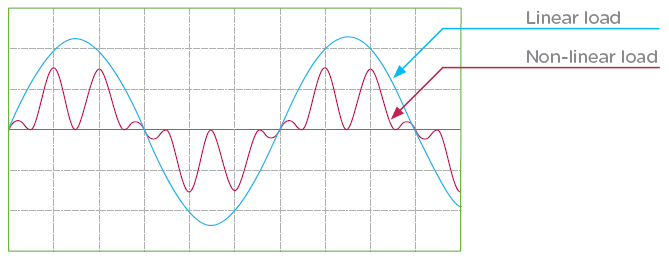
\includegraphics[width=0.7\textwidth]{figure/nonLinear}
	\caption{Lineær belastning sammenlignet med en ulineær belastning.}
	\label{fig:nonLinear}
\end{figure}
%kilde til billede: http://www.sustainableplant.com/2011/when-power-quality-eats-into-energy-efficiency/?show=all

I den virkelige verden er der tilsluttet en lang række ulineære belastninger til elnettet, i form af elektriske strømforsyninger, lysdæmpere, elektronik, frekvensomformer mm. Alle disse trækker strøm i pulser, som forårsager, at elnettes sinussignal bliver forvrænget. Det forvrængede sinussignal giver anledning til større tab i transmissionslinjer, beskadigede komponenter og tab af energi i form af varmeudvikling i transformere og generatorer. \newline

Forvrængningen af sinussignalet kan analyseres ved hjælp af en matematisk funktion kaldet Total Harmonic Distortion (THD). Ved at anvende Fourier-analyse på det forvrængede signal, kan man udlede indholdet af harmoniske. THD er et udtryk for, hvor stor en procentdel de harmoniske svingninger svarer til i forhold til den fundamentale frekvens. Udregningen af THD er givet i formel \ref{eq:THDgenerel}, hvor $V_1$ er amplituden af den fundamentale frekvens. $V_n$ er amplituden af de fortløbende harmoniske. 
\begin{align}
THD = \dfrac{\sqrt{\sum_{n=2}^{\infty}V_n^{2}}}{V_{1}}
\label{eq:THDgenerel}
\end{align}
THD udregnes for spændingen, da det er denne, som er fælles for alle komponenter på elnettet. Teoretisk set indeholder vekselstrømsnettet kun de ulige harmoniske, altså 1, 3, 5 osv. I balancerede systemer kan der også ses bort fra harmoniske, der kan deles med tre, altså 3, 9, 15 osv. Men da elnettet i virkeligheden sjældent er balanceret, er det vigtigt at være opmærksom på, at disse harmoniske kan opstå. \newline

Hvis problemet med harmoniske når til et kritisk niveau, kan systemet analyseres for at finde kilden til forvrængningen og herefter fjerne denne. Der findes også filterkomponenter, som kan minimere transmissionen af harmoniske på elnettet. Disse filtre findes som analoge, der består af spoler og kondensatorer, der dæmper de høje frekvenser. Der findes ligeledes digitale filtre, som analyserer forvrængningen og genererer inverse signaler for at ophæve de harmoniske.\cite{HarmoniskeFiltre}\newline


Kildehenvisning: \cite{HarmoniskeVideo}
 

